\documentclass{article}
\usepackage[utf8]{inputenc}
\usepackage{multicol}
% maxamize space on paper
\usepackage[nomarginpar, margin=.1in]{geometry}
\usepackage{sectsty}
\usepackage{amsmath}
\usepackage{tikz} 
\sectionfont{\fontsize{9}{9}\selectfont}
\subsectionfont{\fontsize{9}{9}\selectfont}
\subsubsectionfont{\fontsize{9}{9}\selectfont}
\usepackage[compact]{titlesec}
\usepackage{enumitem}
\setlength{\parindent}{0pt} 
\setlist[1]{itemsep=-5pt}
\setlist[2]{itemsep=-5pt} 
\begin{document}
\underline{This document is currently incomplete - Information may be incorrect - Please contribute on GitHub!}

\section{P, NP, NP-Completness}

\underline{P:} Generally refers to problems that can be solved in polynomial time

\underline{NP:} Generally refers to problems that can have their solution verified in polynomial time. To show if a problem is NP, show a solution and a verifier.

\underline{NP-Complete:} A problem in NP in which a polynomial-time algorithm that can reduce
the it into any other NP-Complete problem. To prove NP-complete, prove that it is NP and reduce another NP problem to it.

\underline{NP-Hard:} A set of problems that are hard to solve and verify, with some problems not being decideable. Reducable to any problem in NP. To prove, reduce a known NP-complete problem to it in polynomial time.

\underline{P vs NP:} The P vs NP problem is an unsolved problem on whether a problem whose solution can be
verified in polynomial time can also be solved in polynomial time. 

\underline{Vertex Cover:} Set of vertices is a vertex cover if every edge has an endpoint within the
set.

\underline{Independent Set:} Set of vertices is an independent set if no two vertices in the set
share an edge. Related to V.C.: |V.C.| = V - |I.S.|

\underline{Set Cover:} Collection of sets whose union is all the elements in the set of sets.


\underline{Proving NP-X via reduction:} If we wanted to prove that Problem B is NP-X
, we would reduce Problem A (which is known to be NP-X) to it ($A \leq_p B$). 

$Y \le_p X$ means "reducible in polynomial time to" or "$X$ is at least as hard as $Y$. This is proven by reducing $Y$ to $X$

Reduction is done by showing that Y can be solved using a polynomial number of steps and a
polynomial number of calls to a black box that solves X. Proved using a bijection showing that the
reduced version of Y is an instance of X and vice versa.

\underline{Satisfiability/SAT/3-SAT} A formula consisting of clauses with 3 literals per clause.
Between clauses are ANDs and between literals are ORs. The formula is satisifiable if I can make it
true. It is NP-Complete.

\section{Graph Coloring}
Given a graph $G = (V, E)$, find the smallest number of different colors to assign for 
each nod ein $G$ so that no two nodes of the same color share an edge. Decision version: 
Given a graph $G$ and a bound $k$, does $G$ have k-coloring?

Simple when $k=2$ since you just need to check if $G$ is bipartite
When $k=3$, we must prove that it is NP-Complete by reducing 3-SAT to it (3-SAT $\leq_p$ 3-Coloring)

Can be extended to k-Coloring: Add dummy vertices and extra colors accordingly.
\subsection{Hamiltonian Path (NP-Hard)}
Does a graph $G = (V, E)$ have a path $P$ such that for all $v$ in $V$, $v \in P$?
Typically when reducing a problem to hamiltonian path, we want to add 2 extra verticies denoting
where we want the path to start and end. If we wanted to test if there is a hamiltonian path from 
$v_0$ to $v_5$, then we would create nodes $s$ and $t$ and create edges $(s, v_0)$ and $(v_5, t)$
and then check if a path from $s$ to $t$ exists. A hamiltonian cycle is a path that ends at the
start.

\section{Approximation}
\underline{Linear Programming:} Given a set of inequalities that represent constraints, our
goal is to minimize or maxamize a certain quantity represented 
by an equation.
$N<1$-approximations are typically used to represent maxamization problems while
an $N>1$-approximation is typically used to represent a minimization problem. 
$N$-approximation means that the solution is within $OPT*N$

In order to do this, find the worst case and then find a way to relate it to the best case.
A good way to do this is to try to think of inputs that would be really bad for the algorithm
and then try to deduce why it may be bad

General idea: Find the bounds for T* and try to relate them to T.

Maximization: T*/T $\leq$ k

Minimization: T/T* $\leq$ k

\subsection{Load Balancing (NP-Hard)}
This problem is an example for an approx. algorithm. Given $M$ machines $m_1, m_2, ..., m_n$ and $n$ jobs where each job $j$ has a processing time
$t_j$, assign each job to a machine and balance the loads across all machines.

\subsection{Representing Vertex Cover as ILP (Integer Linear Programming)}
Create a function where $x_i = 1$ if the $i^{th}$ vertex is in the cover and 0 otherwise. We'd then multiply this by the weight of node i (if we're doing 
weighted VC), have an objective function where we want $F = \sum_{i=1}^{n} (x_i * w_i)$ to be as small as it can be, and add the constraint 
that for every edge (u,v) that $x_u + x_v \geq 1$ and then we ask ILP to find a solution that satisfies these constraints and minimizes $F$ 

The $x_u + x_v \geq 1$ part ensures that it's a valid cover, since it requires that at least node on each edge is in the cover

The $F= \sum_{i=1}^{n} (x_i * w_i)$ ensures that it's a (somewhat) efficient solution

If unweighted, then $F= \sum_{i=1}^{n} (x_i )$ 

\section{PSPACE and PSPACE-Completeness}
$P \subset NP \subset PSPACE \subset $ everything else\\
PSPACE is the set of decision problems that can be solved by a Turing Machine with a polynomial amount of
space. 

PSPACE-Completeness refers to a PSPACE problem in which every other PSPACE problem could be transformed to it in 
polynomial time

P, NP is solvable in PSPACE. Unknown if NP = PSPACE.

One example: QSAT. Like SAT but the literals are exchanged between either-or and for-all.

\section{Turing Machines}
A turing machine is an abstract machine that given enough time and space can solve any problem. It
is typically represented as a list of cells that has a head which moves to a certain cell, reads a value
and then depending on it's state, usually denoted by $q_n$, it decides what to write to the current cell,
and where to move the head next. The list of states and their outputs can be represented as a series of functions, 
or it can be represented visually as a FSM (Finite State Machine) where each state has a vertex on a graph, and the
possible actions based on the value of the current cell is represented as an edge that specifies direction and then 
some next state. We can represent the state of a turing machine as a list of the cells, with the head at the position
before the cell it is currently reading. The head will be represented by a symbol which represents the current state.
A Turing machine loops forever unless it reaches either the accept or reject
state.

\begin{multicols}{2}
    

For example, these plain english instructions:

State $q_0$:

If cell has value $a$ then go to state $q_0$ and set cell to $b$ and do not move head.

If cell has value $b$ then go to state $q_1$ and move to the right one cell.

State $q_1$:

If cell has value $b$ then go to state $q_0$ and set cell to $a$

If cell has no value ($\sqcup$) then go to state $q_1$ and set the cell to $a$

If cell has value $a$ then go to state $q_{accept}$ (i.e. HALT)

\columnbreak

Can be represented by the functions:


$\delta(q_0, a)  = (q_0, b, /)$

$\delta(q_0, b)  = (q_1, /, R)$

$\delta(q_1, b)  = (q_0, a, /)$

$\delta(q_1, \sqcup)  = (q_1, a, /)$

$\delta(q_1, a)  = (q_accept, /, /)$

\end{multicols}

This can also be represented by the following FSM:

\begin{multicols}{2}
    

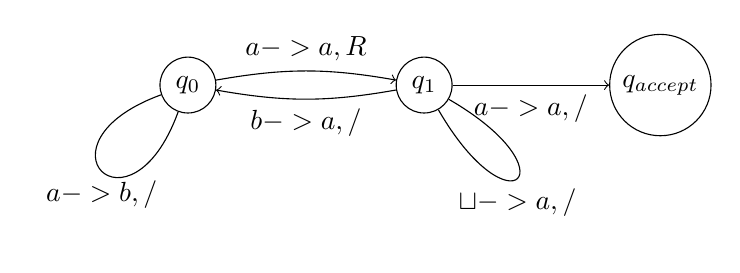
\begin{tikzpicture}[node distance={30mm}, main/.style = {draw, circle}] 
    \node[main] (0)  {$q_0$};
    \node[main] (1) [right of=0] {$q_1$};
    \node[main] (2)  [right of=1] {$q_{accept}$};

    \path [->,bend left=10] (0) edge node [above] {$a -> a, R$} (1);
    \path [->,bend left=10] (1) edge node [below] {$b -> a, /$} (0);
    \path (1) edge [out=330,in=300,looseness=25] node[below] {$\sqcup -> a, /$} (1);
    \path (0) edge [out=200,in=250,looseness=15] node[below] {$a -> b, /$} (0);
    \path [->] (1) edge node [below] {$a -> a, /$} (2);
\end{tikzpicture}

\columnbreak

So a machine in the state $q_0 a \sqcup\sqcup$ would transition through the following states:

$q_0 a \sqcup\sqcup$

$q_0 b \sqcup\sqcup$

$a q_1 a\sqcup$

$a q_{accept} a\sqcup$

\end{multicols}

\subsection{Formal languages/Recognizability}
A formal language is a set of strings which are a finite sequence of symbols from an alphabet. And
alphabet is a finite set of symbols.

A language is recognizable if a Turing machine can be constructed that will accept all strings in
the language. It is decidable if all inputs halt.

A universal Turing machine is a Turing machine that can simulate another.

\section{Undecidability and Halting problem}
An undecidable problem is a problem in which no algorithm can produce a correct response on every
input. In order to prove a problem is undecidable, we can reduce another undecidable problem to it, 
or we can use a proof by contradiction by specifying a scenario in which it wouldn't be possible
to return a correct result (how the Halting problem is commonly proved).

The halting problem is an undecidable problem that takes a function and some input as input. It then returns
wether this program will run forever or if it will eventually halt. It is undecidable because a theoretical
function $C(X) -> if H(X,X) == 'HALT' then LOOP else HALT$ would generate an incorrect output if $C(C)$ is called.


\section{Randomized Algorithms}
Expectance is equal to a value multiplied by the chance that that that value will occur
(this is the average value taken by a random variable)$E(x) = \sum XP(X)$


\subsection{Randomized Median Finding Runtime Summary}
The proof shows that the randomized algorithm has an expected running time of $\frac{1}{4}cn + O(n)$, where $c$ is a constant. This is faster than the worst-case running time of the deterministic algorithm, which is $O(n^2)$, under certain assumptions about the distribution of the input. Thus, on average, the randomized algorithm is faster than the deterministic algorithm for finding the median of an unsorted list.


\section{Misc}



\end{document}
